\chapter[Przegląd czujników ultradźwiękowych]{Przegląd czujników ultradźwiękowych}

\label{chapter:przeglad_czujnikow}



% Proszę opisać kilka wybranych, możliwie reprezentatywnych
% dalmierzy ultradźwiękowych.

\section{Dobór odbiornika}
Wymagania jakie powinien spełniać odbiornik wynikają bezpośrednio z założeń projektu. 
Pierwszym z nich jest zakres pasma przenoszenia czujnika który obejmie częstotliwość \unit[40]{kHz} na akceptowalnym poziomie sygnału, 
czyli takiej częstotliwości na jakiej pracuje w rezonansie większość nadajników piezoelektrycznych dostępnych na rynku. 

\begin{figure}[ht!]
    \centering
    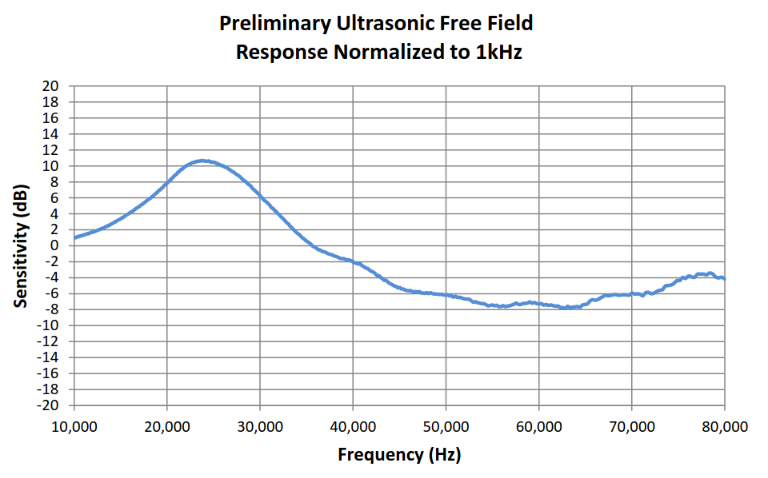
\includegraphics[width=0.5\textwidth]{mic_response.png}
    \caption{Pasmo przenoszenia mikrofonu SPU0410LR5H-QB}
    \label{fig:}
\end{figure}
\noindent
Następnym wymaganiem jest rozmiar, by móc interpolować kierunek przyjścia sygnału w zakresie $180^\circ$, 
odległość między odbiornikami nie powinna przekraczać pół długości fali czyli \unit[4,25]{mm}\footnote[1]{W powietrzu, w temperaturze 15 °C, prędkość rozchodzenia się dźwięku jest równa 340,3 m/s \cite{sound_speed}}
Wszystkie czujniki tak małych rozmiarów są produkowane w technologii MEMS. 
\begin{figure}[ht!]
    $$\lambda = \frac{v}{f} = \frac{340,3\frac{m}{s}}{40kHz}=0,0085m = 8,5mm$$
\caption{Obliczenie długości fali}    
\end{figure}
\noindent
Kolejnym wymaganiem jest takie umieszczenie otworu ciśnieniowego w obudowie, by skierowany był on wewnątrz laminatu obwodu drukowanego. 
Taka konstrukcja pozwala na stworzenie płaskiej powierzchni tylko z otworami ciśnieniowymi czujników, 
co przekłada się na mniejsze zakłócenia spowodowane odbiciami fali dźwiękowej od elementów elektronicznych.

\begin{figure}[ht!]
    \centering
    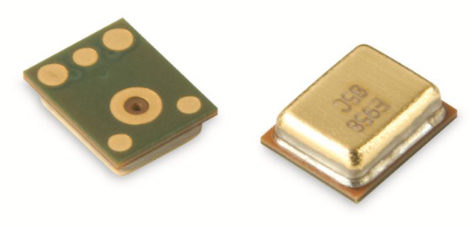
\includegraphics[width=0.5\textwidth]{mic.png}
    \caption{Mikrofon SPU0410LR5H-QB}
    \label{fig:mic}
\end{figure}
\noindent
Ostatecznym wymaganiem była dostępność i przystępność cenowa produktu. Ze względu na tak rygorystyczne oczekiwania wybór zawęził się zaledwie do kilku pozycji.
Jedną z nich był mikrofon SPU0410LR5H-QB marki Knowles\cite{knowles}, który w odpowiedniej ilości został dostarczony przez Promotora.



\section{Komercyjne rozwiązania}
Na rynku znajduje się bardzo dużo ultradźwiękowych czujników odległości, ale wzglednie niewiele firm oferuje sonary bez ruchomych elementów.
Czołowym producentem urządzeń w takiej technologii jest TOPOSENS ze swoim produktem o nazwie ECHO ONE\textregistered.
Zdjęcia produktu sugerują, że posiada on ultradźwiękowy nadajnik oraz trzy odbiorniki we wzorze tworzącym kąt prosty.

\begin{figure}[ht!]
    \centering
    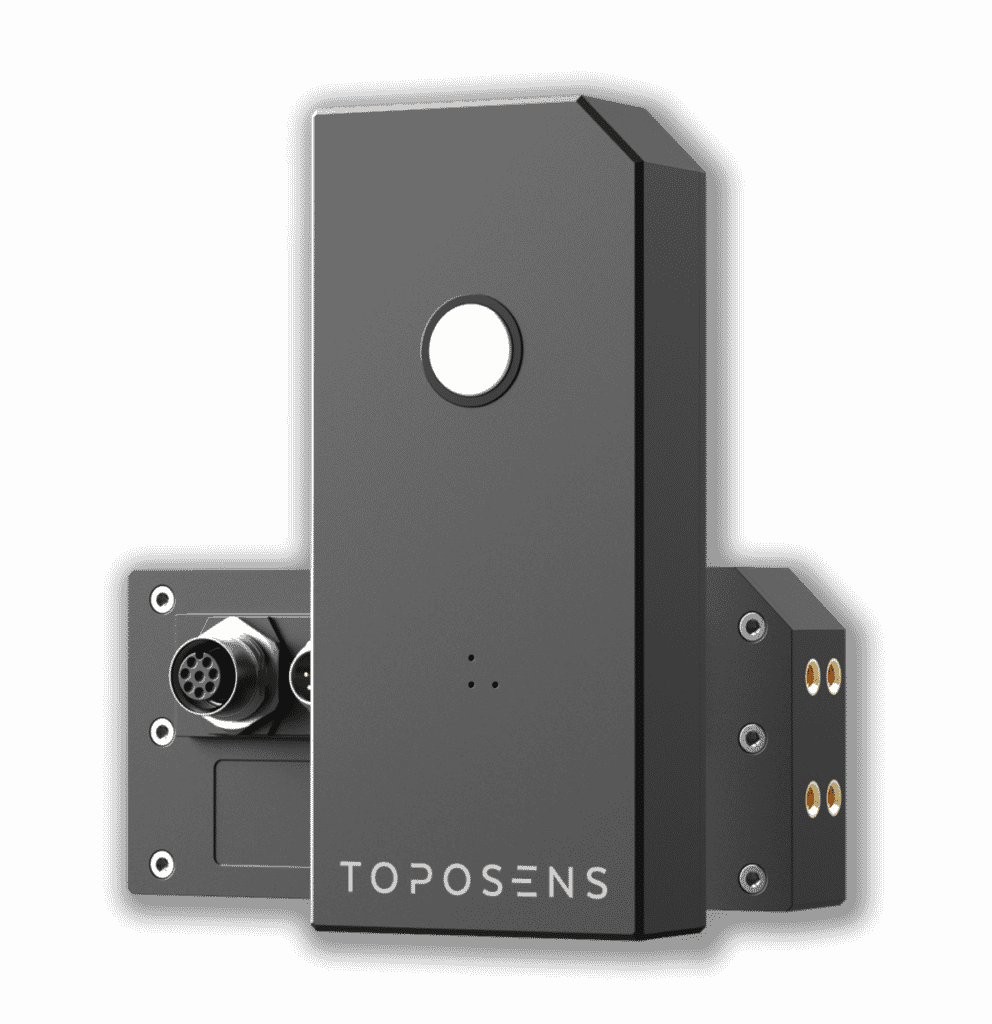
\includegraphics[width=0.3\textwidth]{ECHOONE.png}
    \caption{TOPOSENS ECHO ONE}
    \label{fig:echoone}
\end{figure}

\todo{dodać źródło obrazka}